\subsection{Pictures}

For an idea generation process we all sat around the same table and passed around pictures. We started with the pictures face down so we would pick them at random. When passing the pictures around, each of us said what came to mind when looking at the pictures, always keeping in mind that we were to make a creative functional robot. We made sure not to comment on each others thoughts so all thoughts were allowed. 




It was very interesting to see how different pictures generated different thoughts. There was a picture of an opera singer, and the thoughts there were: "Loud", "Hard work", "Love for your work", "Human interaction", "Service provider", "Sound recognition" and "Training algorithms". 
Another picture was of a cellphone and the thoughts there were: "Interface", "Monitoring", "Portability", "Connectivity", "Extension/Multi-functional", "Compact", "User experience", "New experience", and "Awareness/focus". 

\begin{figure}[ht]
\centering
  \begin{subfigure}[b]{0.3\textwidth}
    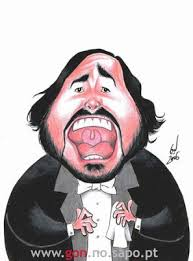
\includegraphics[width=\textwidth]{./graphics/pavarotti}
    \caption{Picture of opera singer used in the idea generating process.}
    \label{fig:pavarotti}
  \end{subfigure}
  \begin{subfigure}[b]{0.3\textwidth}
    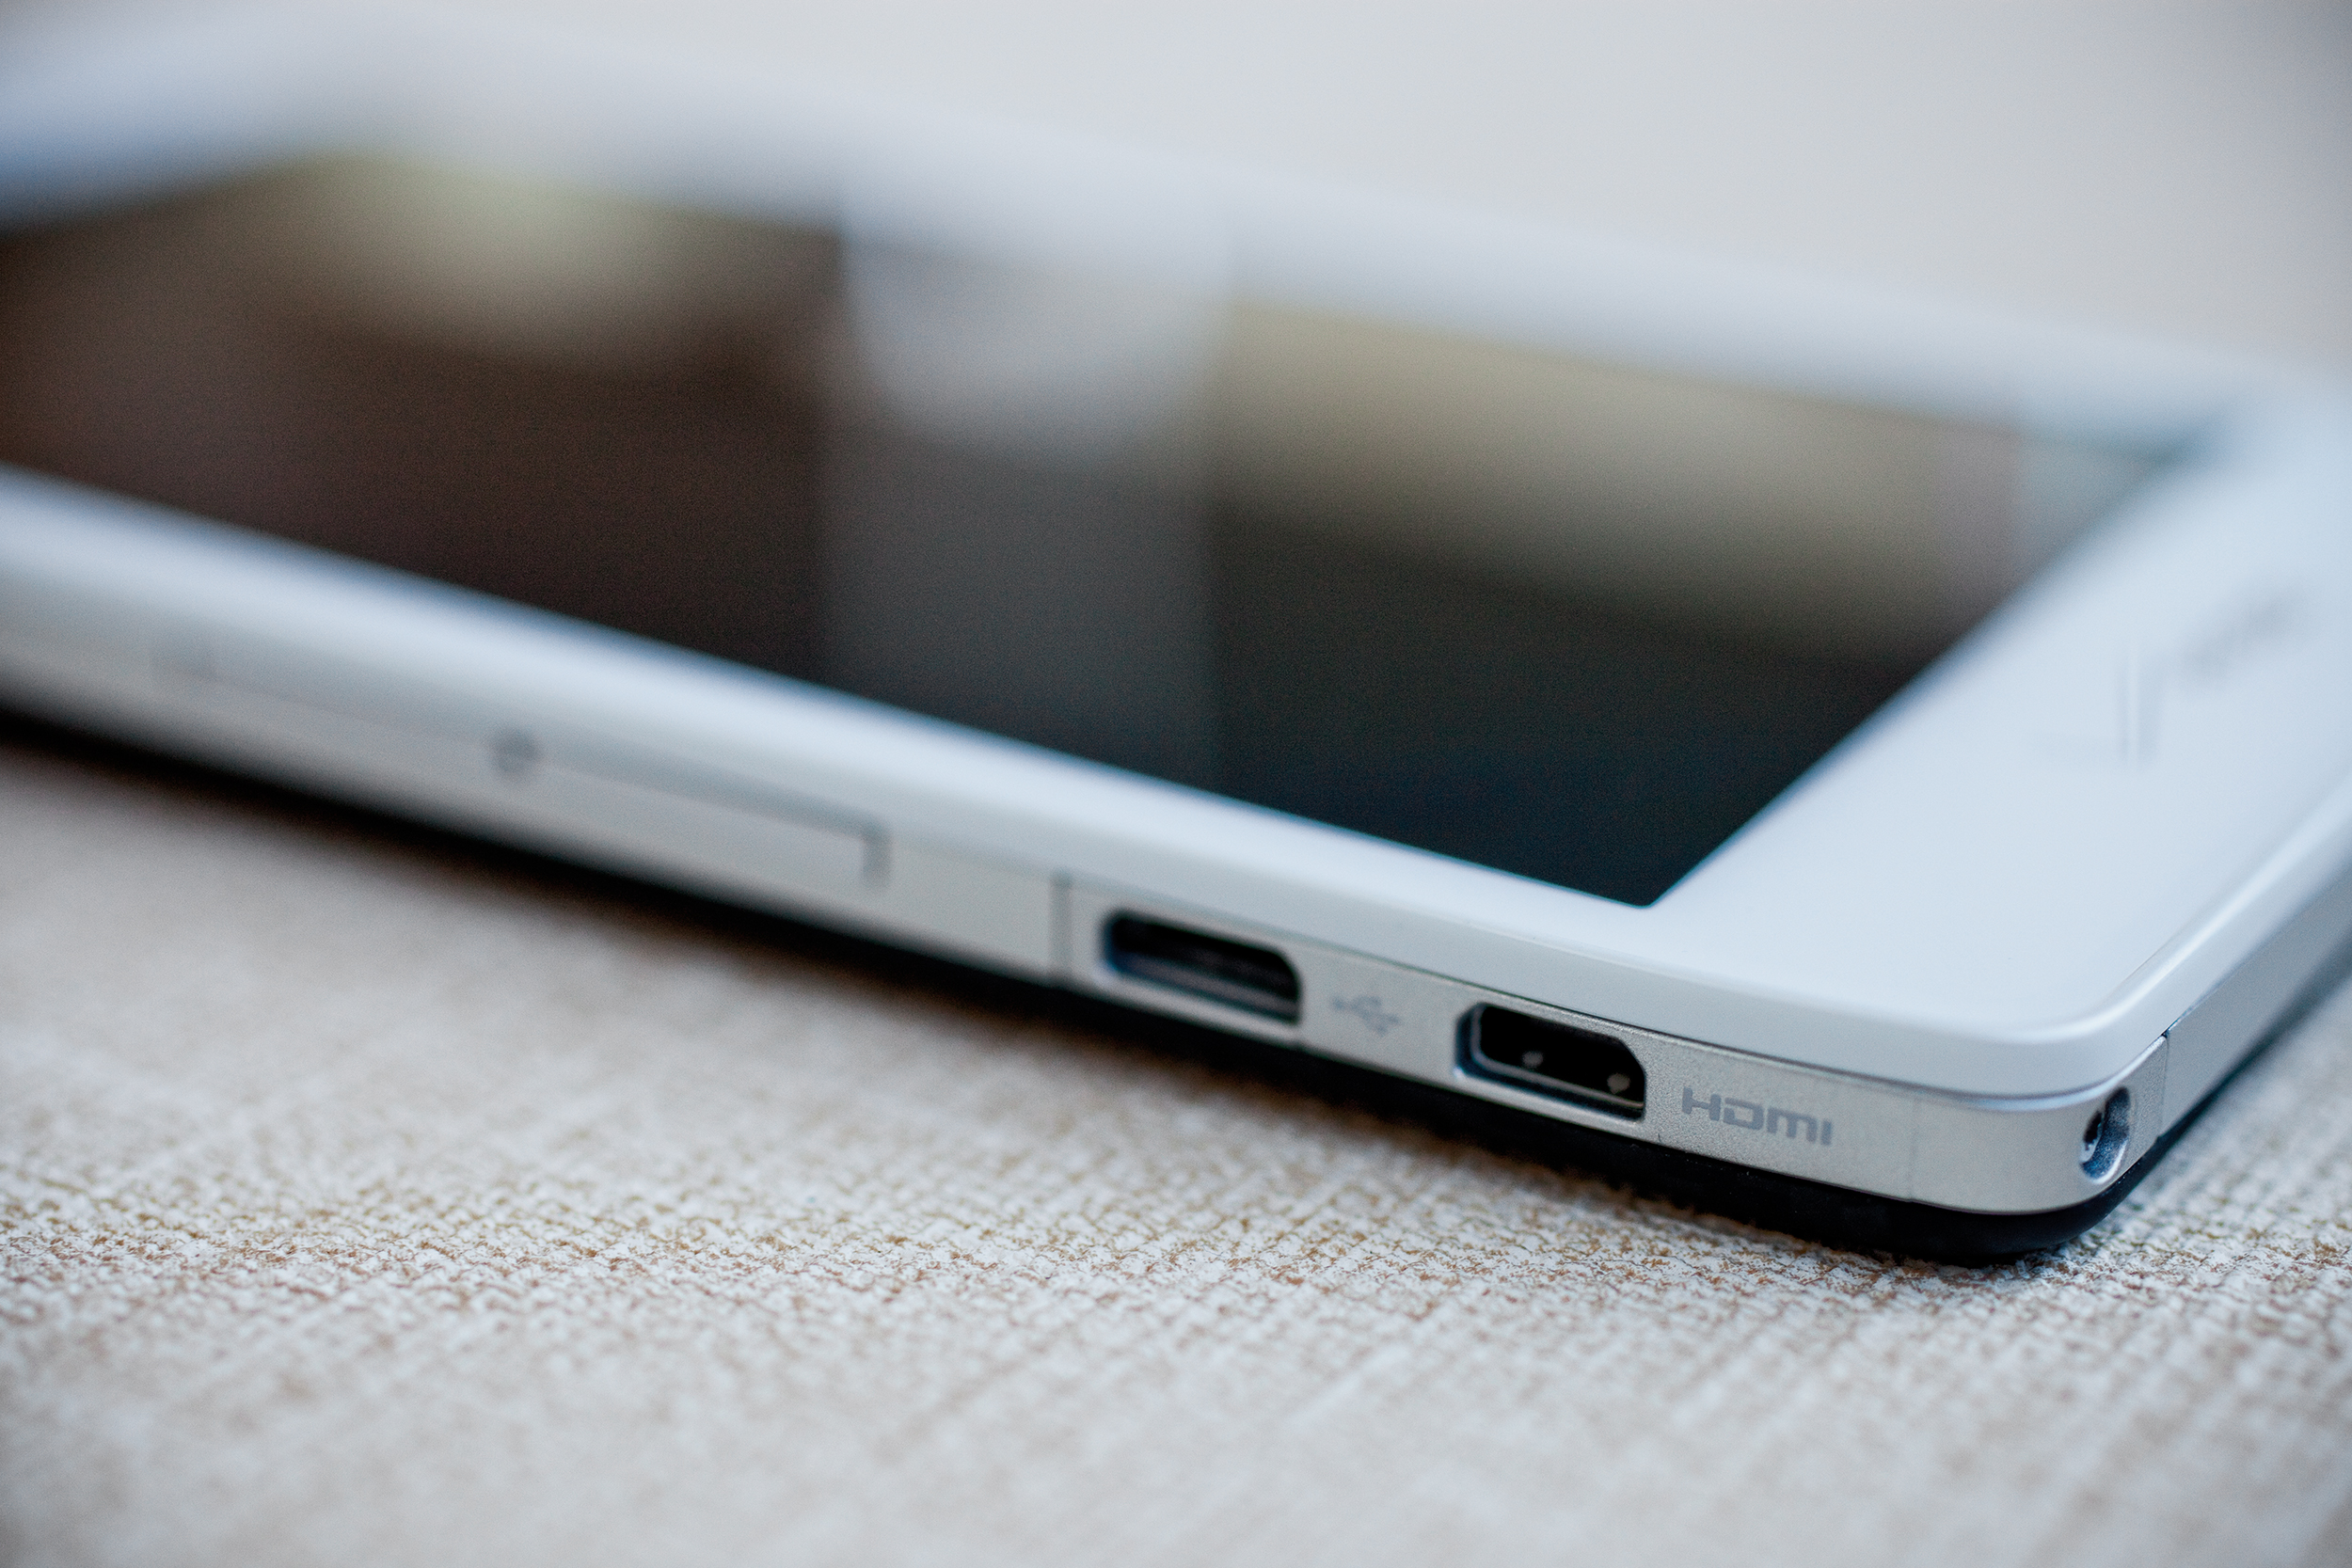
\includegraphics[width=\textwidth]{./graphics/phone}
    \caption{Picture of cellphone used in the idea generating process.}
    \label{fig:phone}
  \end{subfigure}
\caption{Pictures used in the idea generating process}
\end{figure}





In the beginning of this process several of us found it to be somewhat a waste of time. It was difficult to see how a picture of an opera singer should help us design a robot. After the process, however, we all agreed that we had come up with some really good words, and a lot of them were words that we would like to describe our product, e.g.: "Mobility", "Safety", "Combined knowledge", "Service provider" and "Precision". Other words we would have to make sure would not end up describing our product, e.g.: "Loud", "Danger", and "Legal issues". 